% Introduction
\subsection*{Introduction}
Through the development of AlphaZero, a general model for board games with superhuman ability has 
been achieved in three games: Go, chess, and Shogi. It could achieve these results without the need for 
human gameplay data or history, instead using self-play in an enclosed environment. However, the 
model still relied on a simulator that could perfectly replicate the behavior, which might not translate 
well to real-world applications, where modeling the system might not be feasible. MuZero 
was developed to address this challenge by developing a model-based RL approach that could learn 
without explicitly modeling the real environment. This allowed for the same general approach used in 
AlphaZero to be used in Atari environments where reconstructing the environment is costly. Essentially, 
MuZero was deployed to all the games with no prior knowledge of them or specific optimization and 
managed to show state-of-the-art results in almost all of them.

% MuZero Algorithm
\subsection*{MuZero Algorithm}
\begin{figure}[h!]
    \centering
    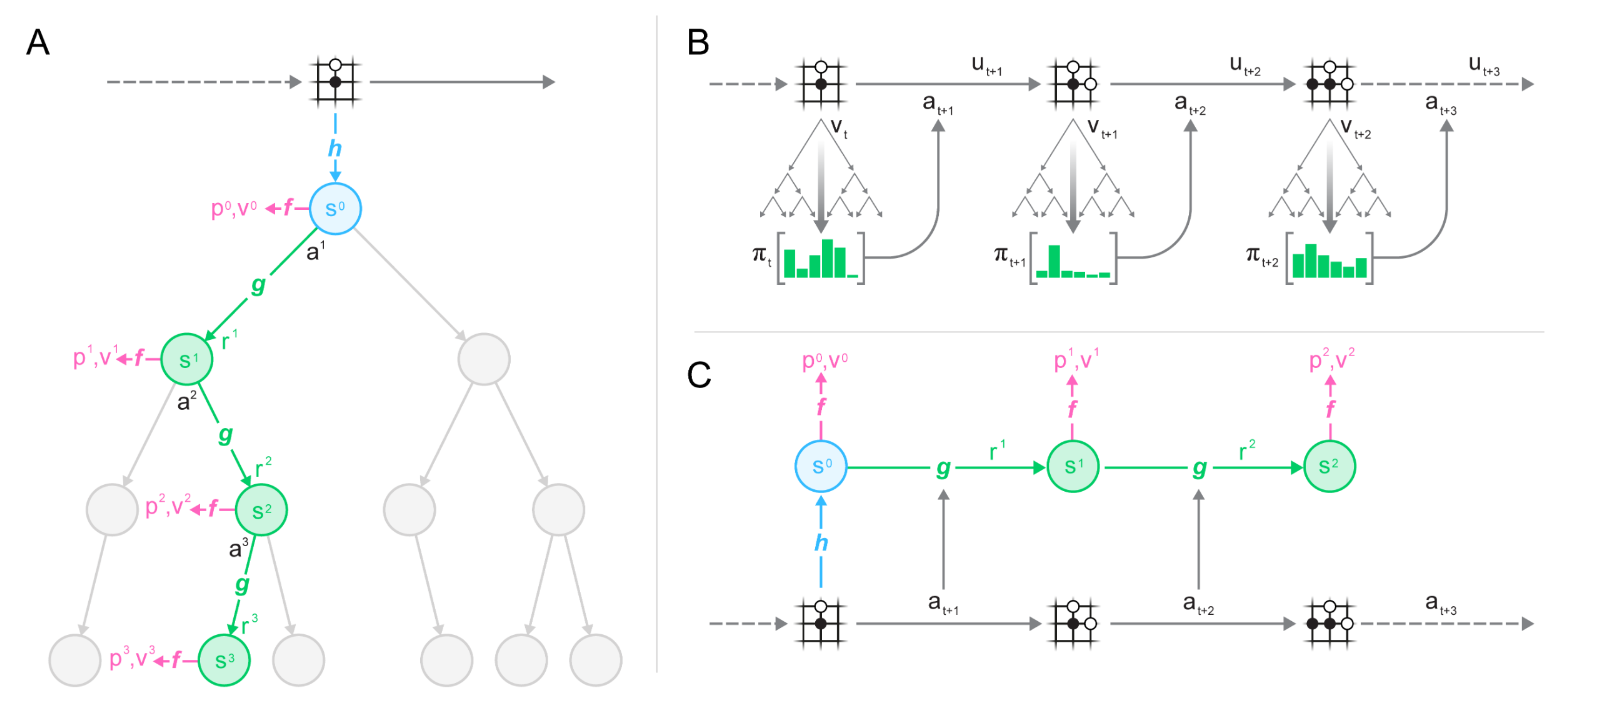
\includegraphics[width=0.35\textwidth]{sections/6MuZero/graph_1.png}
    \caption{This is a sample image.}
    \label{fig:(A)The progression of the model through its MDP. (B)MuZero acting as an environment with MCTS as feedback. (C)A diagram of training MuZero's model}
\end{figure}
The model takes in an input of observations $o_1, \ldots, o_t$ that are then fed to a representation network $h$, 
which reduces the dimensions of the input and produces a root hidden state $s_0$. Internally, the model 
mirrors an MDP, with each state representing a node with edges connecting it to the future states 
depending on available actions. Unlike traditional RL approaches, this hidden state is not constrained to
contain the information necessary to reproduce the entire future observations. Instead, the hidden states 
are only optimized for predicting information that is related to planning. At every time step, the model 
predicts the policy, the immediate reward, and the value function. The output of the state-action pair is 
then used by the dynamics function to produce future states. Similar to AlphaZero, a Monte Carlo tree 
search is used to find the best action policy given an input space. This is used to train the model by 
comparing the MCTS policy with the predictor function policy. Also, after a few training runs, the model 
ceases to use illegal moves, and the predicted actions map to the real action space. This eliminates the 
need for a simulator, as the model internalizes the environment characteristics it deems necessary for
planning and acting, which generally converges to reality through training. The value function at 
the final step is compared against the game result in board games, i.e., win, loss, or a draw.

% Insert Equations Here
\subsection*{Equations}
\begin{align}
    s_0 &= h_\theta(o_1, \ldots, o_t) \\
    r_k, s_k &= g_\theta(s_{k-1}, a_k) \\
    p_k, v_k &= f_\theta(s_k) \\
    \begin{bmatrix}
        p_k \\ v_k \\ r_k
    \end{bmatrix} 
    &= \mu_\theta(o_1, \ldots, o_t, a_1, \ldots, a_k)
\end{align}

\begin{align}
    \nu_t, \pi_t &= \text{MCTS}(s_0^t, \mu_\theta) \\
    a_t &\sim \pi_t
\end{align}

\begin{align}
    p_k^t, v_k^t, r_k^t &= \mu_\theta(o_1, \ldots, o_t, a_{t+1}, \ldots, a_{t+k}) \\
    z_t &= 
    \begin{cases} 
        u_T & \text{for games} \\
        u_{t+1} + \gamma u_{t+2} + \ldots + \gamma^{n-1} u_{t+n} + \gamma^n \nu_{t+n} & \text{for general MDPs}
    \end{cases} \\
    l_t(\theta) &=
    \sum_{k=0}^K \big[ l_r(u_{t+k}, r_k^t) + l_v(z_{t+k}, v_k^t) + l_p(\pi_{t+k}, p_k^t) \big] 
    + c \|\theta\|^2
\end{align}

\begin{align}
    l_r(u, r) &= 
    \begin{cases} 
        0 & \text{for games} \\
        \phi(u)^T \log r & \text{for general MDPs}
    \end{cases} \\
    l_v(z, q) &=
    \begin{cases} 
        (z - q)^2 & \text{for games} \\
        \phi(z)^T \log q & \text{for general MDPs}
    \end{cases} \\
    l_p(\pi, p) &= \pi^T \log p
\end{align}

% MCTS
\subsection*{MCTS}
MuZero uses the same approach developed in AlphaZero to find the optimum action given an internal 
state. MCTS is used where states are the nodes, and the edges store visit count, mean value, policy, and 
reward. The search is done in a three-phase setup: selection, expansion, and backup. The simulation 
starts with a root state, and an action is chosen based on the state-transition reward table. Then, after the end 
of the tree, a new node is created using the output of the dynamics function as a value, and the data from the 
prediction function is stored in the edge connecting it to the previous state. Finally, the simulation 
ends, and the updated trajectory is added to the state-transition reward table. In two-player zero-sum 
games, board games, for example, the value function is bounded between 0 and 1, which is helpful to 
use value estimation and probability using the pUCT rule. However, many other environments have 
unbounded values, so MuZero rescales the value to the maximum value observed by the model up to 
this training step, ensuring no environment-specific data is needed.

% Results
\subsection*{Results}
The MuZero model demonstrated significant improvements across various test cases, achieving state-of-the-art performance in several scenarios. Key findings include:

\subsubsection*{Board Games}
\begin{itemize}
    \item When tested on the three board games AlphaZero was trained for (Go, chess, and shogi):
    \begin{itemize}
        \item MuZero matched AlphaZero's performance \textbf{without any prior knowledge} of the games' rules.
        \item It achieved this with \textbf{reduced computational cost} due to fewer residual blocks in the representation function.
    \end{itemize}
\end{itemize}

\subsubsection*{Atari Games}
\begin{itemize}
    \item MuZero was tested on 60 Atari games, competing against both human players and state-of-the-art models (model-based and model-free). Results showed:
    \begin{itemize}
        \item \textbf{Starting from regular positions:} MuZero outperformed competitors in \textbf{46 out of 60 games}.
        \item \textbf{Starting from random positions:} MuZero maintained its lead in \textbf{37 out of 60 games}, though its performance was reduced.
    \end{itemize}
    \item The computational efficiency and generalization of MuZero highlight its effectiveness in complex, unstructured environments.
\end{itemize}

\subsubsection*{Limitations}
\begin{itemize}
    \item Despite its strengths, MuZero struggled in certain games, such as:
    \begin{itemize}
        \item \emph{Montezuma's Revenge} and \emph{Pitfall}, which require long-term planning and strategy.
    \end{itemize}
    \item General challenges:
    \begin{itemize}
        \item Long-term dependencies remain difficult for MuZero, as is the case for RL models in general.
        \item Limited input space and lack of combinatorial inputs in Atari games could introduce scalability issues for broader applications.
    \end{itemize}
\end{itemize}

